\documentclass[a4paper]{article}

\input ../header
\usepackage[np]{numprint}

\setlength{\multicolsep}{2pt}

\begin{document}

\title{Sujet A -- La photographie numérique}

\pagestyle{empty}

\date{}
\author{}

\maketitle{}
\thispagestyle{empty}

% QCM histoire de la photographie numérique
\exo[4 points] Cet exercice est un QCM. Pour chaque question posée, une seule des réponses proposées est correcte. Entourer sur l'énoncé la réponse que vous pensez être correcte.\\
Une bonne réponse rapporte 1 point, une mauvaise réponse ou l'absence de réponse ne rapporte  ni n'enlève aucun point. Le fait d'entourer plusieurs réponses pour une question donnée rapporte 0 point.

\begin{enumerate}
  \item Les photorécepteurs situés dans la rétine s'appellent les :
    \begin{multicols}{4}
      \begin{enumerate}
	\item photosites
	\item cônes
	\item filtres
	\item lumino-capteurs
      \end{enumerate}
    \end{multicols}
  \item Dans une image numérique, un pixel :
    \begin{multicols}{4}
      \begin{enumerate}
	\item n'a pas de taille prédéfinie
	\item a une taille fixe sur tous les écrans
	\item a une taille variable selon la couleur de l'image
	\item a une taille fixe sur toutes les imprimantes
      \end{enumerate}
    \end{multicols}
  \item La définition d'une image numérique est :
    \begin{multicols}{4}
      \begin{enumerate}
	\item son nombre de pixels 
	\item son degré de netteté
	\item le rapport de sa largeur par sa hauteur (par ex. 16:9 ou 4:3)
	\item exprimée en dpi ou ppp
      \end{enumerate}
    \end{multicols}
  \item Je suis un américain, co-inventeur du capteur CCD. Je suis :
    \begin{multicols}{4}
      \begin{enumerate}
	\item Nicéphore Niepce
	\item Thomas Sutton
	\item Willard Boyle
	\item George E. Smith
      \end{enumerate}
    \end{multicols}
\end{enumerate}

\bigskip

\exo[1 point] Compléter la phrase ci-dessous :

\begin{center}
  \og{}Je suis un composant transformant ce qui est perçu par notre oeil en image numérique. Je suis \dotfill\fg{}
\end{center}

\bigskip

% Calcul de la définition
\exo[3 points] Tumoanatea souhaite imprimer une photo aux dimensions $76,2$ cm $\times$ $63,5$ cm avec une résolution de $200$ dpi. Quelle définition minimale devra avoir le fichier fourni par Tumoanatea ?\rep{10}

\bigskip

\exo[3 points] Expliquer les similitudes entre l'oeil humain et un appareil photo numérique.\rep{8}

\pagebreak

% Calcul de la résolution
\exo[3 points] Voici une publicité pour le Samsung Galaxy S21 Ultra:

\medskip

\begin{multicols}{2}
  \begin{enumerate}
    \item [] 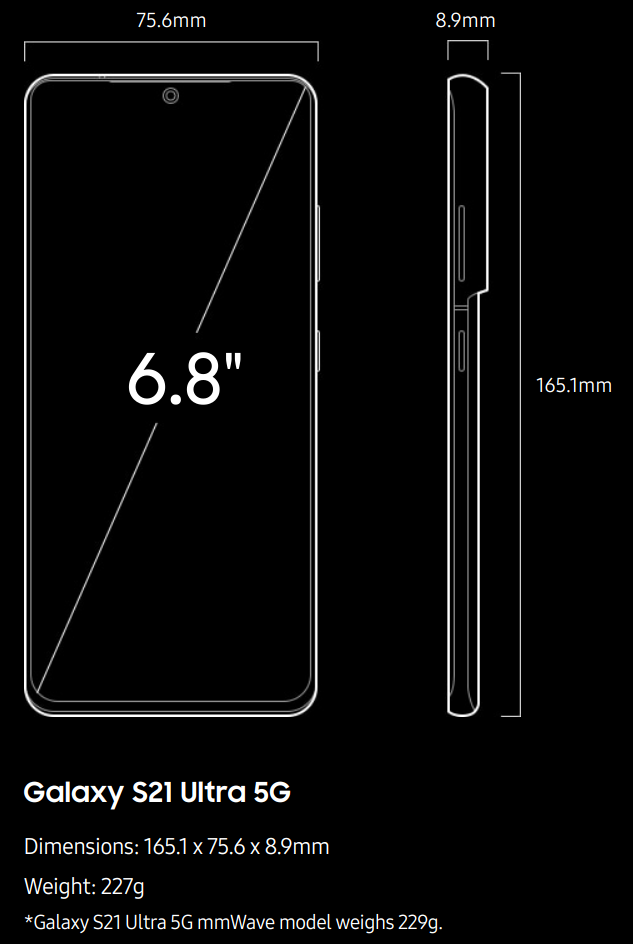
\includegraphics[width=6cm]{evaluation_samsung_galaxy_S21_ultra_1.png}
    \item [] 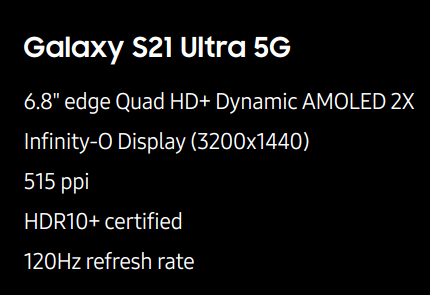
\includegraphics[width=6cm]{evaluation_samsung_galaxy_S21_ultra_2.png}
  \end{enumerate}
  Retrouver, par le calcul, la résolution annoncée.\rep{10}
\end{multicols}

\medskip


\bigskip

% Étude de documents sur le droit à l'image
\exo[3 points] Lire les documents suivants :

\begin{center}
  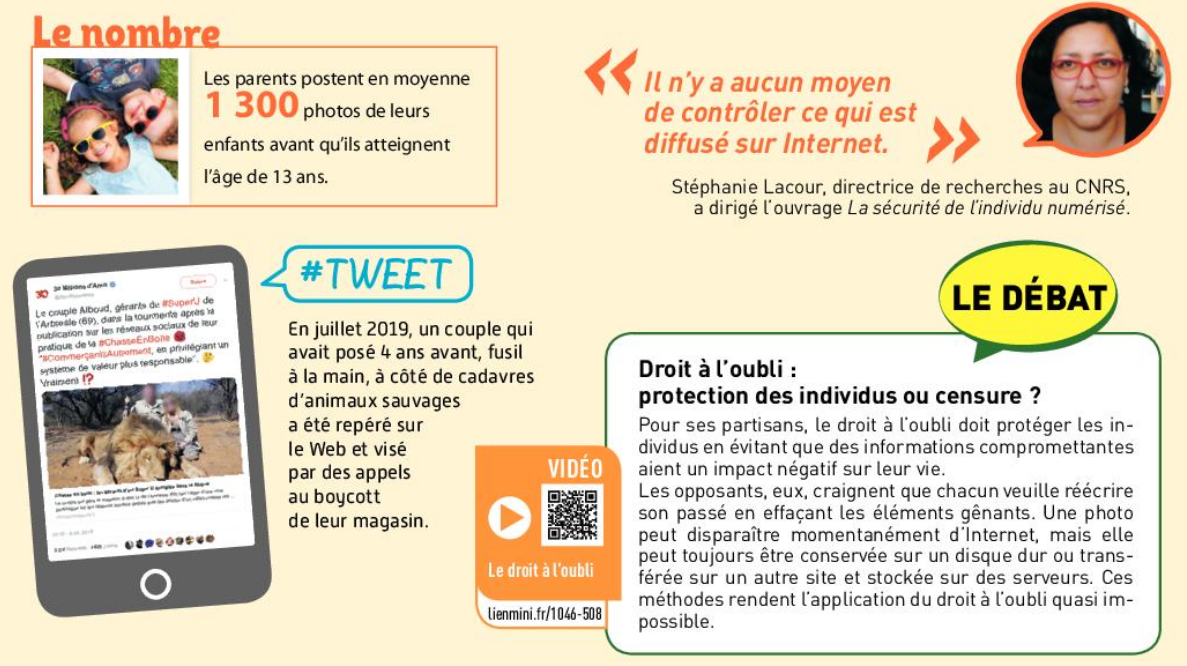
\includegraphics[width=16cm]{evaluation_droit_a_l_oubli.png}
\end{center}

\begin{enumerate}
  \item Compléter le texte suivant :

    \medskip

    Le $\hdots\hdots\hdots\hdots\hdots\hdots$ des données à caractère personnel permet à toute personne de faire $\hdots\hdots\hdots\hdots\hdots\hdots$ une image ou des informations afin de protéger $\hdots\hdots\hdots\hdots\hdots\hdots$ Mais tôt ou tard, ces $\hdots\hdots\hdots\hdots\hdots\hdots$ peuvent ressurgir ce qui re $\hdots\hdots\hdots\hdots\hdots\hdots$ de cette loi très difficile.
  \item Proposer un argument en faveur du droit à l'oubli et un argument contre son application systématique.
    \begin{multicols}{2}
      \begin{enumerate}
	\item Pour\rep{6}
	\item Contre\rep{6}
      \end{enumerate} 
    \end{multicols}
\end{enumerate}

\end{document}
